\chapter{Requirements and Analysis}

\section{Problem Statement}
Having looked at the background information on distributed sytems, consensus protocols
and Disel, we can formalise the problem statement for the project.
The project aims to mechanise the proof of Paxos in
Disel. Mechanisation is a way to use Coq's higher-order logic to build mechanically
checked proofs of the consensus agreement and the code correctness.

This will involve doing the modelling on the protocol to come up with
state transitions and inductive invariants, in order to encode it in Disel.
Additionally, we will also implement a client application built on top
of the verified protocol that uses Disel's code extraction features.

The mechanisation will allow us to prove the inductive invariant for Paxos,
that proves consensus being achieved,
and also show that the implemented client application complies with the protocol.

% Section 3.1 – tell what do you mean  to prove (compliance of implementation to the protocol,
% invariant inductivity etc). Better yet, say that you are formalising Paxos in Disel, so that
% the formalisation will allow you to establish (i.e., prove) the properties mentioned above.
% You can expand on this in requirements, telling what exactly are the logical statements of
% interest wrt. to the system in question (Paxos) that you'd like to prove via encoding it in
% Disel. Also, you should mention that


\section{Requirements}
\begin{enumerate}
  \item Adapt Paxos for encoding in Disel and devise the state-transition system for this protocol.
  \item Develop an inductive invariant for the adapted protocol that
    ensures the protocol functions correctly by imposing requirements on the global state of the system
  \item Implement a simulation of the adapted protocol with the developed state transition system.
  \item Mechanise the proof of the adapted protocol in Disel/Coq.
    Thereby, providing a library of reusable verified distributed components.
  \item Mechanise a client application of the protocol verified out of the abstract interface.
\end{enumerate}

\vspace{-5mm}
\section{Analysis: Approach to Mechanising Proofs in Disel}
Having decided on the requirements we came up with a workflow to
mechanise the proof in Disel. Finishing all the stages in the workflow
will help us to meet all our requirements.

\begin{figure}
\centering
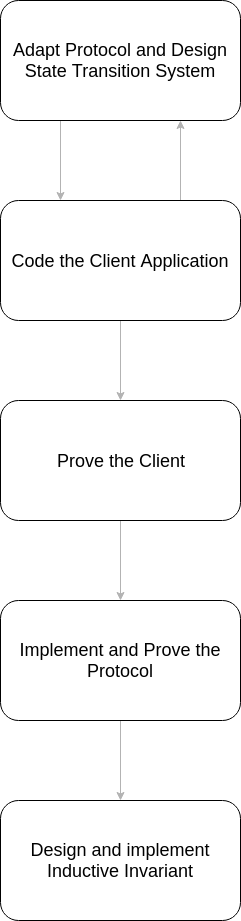
\includegraphics[width=\textwidth]{figures/disel_workflow.png}
\caption{Disel Workflow
\label{fig:myInlineFigure}}
\end{figure}

% (1) Write code before proofs and run/test it;
%         (2) Prove that the code follows the protocol;
%         -----
%         (3) Write the protocol and prove invariants;
%
%
% You might want to have a diagram for this…
%
% Take a look at this paper (without going into details):
%
% https://www2.eecs.berkeley.edu/Pubs/TechRpts/2017/EECS-2017-163.pdf
%
% You might want to make a point that even without verifying inductive invariants, we already can get relatively strong correctness properties just by verifying (1)-(2).
%
% (1)-(2) is also sort of delivered by this work: https://eb.host.cs.st-andrews.ac.uk/writings/tdd-conc.pdf
%
% 1. I suggest you first
%   give a textual description with a lot of intuition about what kind of client
%   we are interested in and what properties it can observe that are guaranteed by the consensus.
% 2. Then you specify this property formally and sketch its proof.
%
% The client application does only need to have a couple of RPC-like procedures.
% It doesn't have to know about the entire protocol.
%
% Adapt Protocol and Design State transition system (iterate)
% | |
% Design and implement the Client Application (iterate)
% |
% Prove Client
% |
% Implement and prove Protocol
% |
% Prove the Inductive Invariant

\subsection{Adapt protocol and design state transition system}
By adapting the protocol we try to focus on the `core' parts of the protocol
and to do away with the `convenience' parts. For Paxos, this is focusing on the
part of the protocol that deals with achieving consensus and not looking at the
part where the learner is informed of the decision.

We also need to design state transition systems for the nodes that participate
in the protocol. This makes it easier for us to encode the protocol in Disel as
we already know which send and receive transitions we will need from each state
and thus can easily code the transition wrappers.

In chapter 4, we look go into the details of how we tackled this stage on our way
to mechanising the proof of Paxos.

\subsection{Code the client application}
Secondly, we need to think of a client application that uses the implemented protocol.
We need to design and implement a client that will demonstrate the properties of the
protocol that we want to prove. In case of Paxos, we will design a client
where nodes try to acheive consensus on one of the proposals that the proposer
is initialised with. This will enabled us to see in action the stages of the protocol
that lead to consensus being achieved.

While using Disel, we will often had to cycle between stage 1 and stage 2.
This is because while implementing the client, you realise things like, you are
missing one state for a node that is required in order for the protocol to progress.
There was a case when we saw this while writing the client for Paxos.
We realised that we were missing the \texttt{PAbort}
state for the proposer, which was necessary to signify when a proposer stops
participating in the protocol.

The process of cycling between stages 1 and 2 allow us to solidify our adapted
protocol. Doing this at an early stage (before starting the proofs)
also has the advantage of us not having to rewrite a lot of code that will also
break all the proofs relating to the change.

Additionally, implementing the client also helps us identify unnecessary stages
and transitions in the adapted protocol which were not needed to implement the
client. Reducing the number of states and transitions vastly reduces the amount
of things you will need to prove in the later stages.

\subsection{Prove the code follows the protocol}
The next stage involves encoding and proving the protocol
and proving that the code for the client actually follows
the adapted protocol. Thus, finishing the proofs in this stage gives us
confidence that our adapted protocol can actually be used to fulfil the role
which our client performs. In case of Paxos, this helped us realise that our
adapted protocol can be used to achieve consensus among the acceptors.
Finishing this stage means that we have finished the proof of the client.
Yet, at this stage we can only be sure that the code follows the protocol.

Reaching this state also gives us relatively strong correctness properties. This
because just by ensuring the code follows the protocol, if the protocol we have
implemented has already been, we can know that the code will work correctly
although we cannot be completely sure until we finish the next stage.
In the mechanising of Paxos we were only able to reach till this stage,
we designed the inductive invariant but ran out of time to encode it.
As the actual protocol we encoded is the simple Paxos algorithm, it still
gives us quite a strong correctness as the simple Paxos algorithm has a proof
of safety and has also been used to implement real world systems.

\subsection{Implement and prove the inductive invariant}
An inductive invariant is necessary as it helps verify the entire
global system. As without it, the code might follow the protocol, but the
protocol might itself be broken. In case of Paxos this could be the case that
the nodes follow the protocol but they never achieve consensus.
